\documentclass{article}
\usepackage[utf8]{inputenc}
\usepackage{gensymb}
\usepackage{graphicx}


\title{Laboratorio 5. Óptica Geométrica}
\author{Carlos Alberto Dagua Conda, Hector Fabio Jimenez Saldarriaga, \\Juan Camilo Castrillon,\thanks{carlosdaguaco@utp.edu.co, hfjimenez@utp.edu.co, jucacastrillon@utp.edu.co} }

\date{Febrero 2016}

\begin{document}

\maketitle

\section{Abstract}

In this paper we study experimentally different phenomena arising in geometrical optics like RBG color model, reflection and refraction. This is approach knowledge to introduce the basic concepts, however there is unknown that the geometrical optics does not account for certain effects such as diffraction and interference.


\section{Introducción}


La Óptica Geométrica fue desarrollada antes de que la luz se describiese como una onda electromagnética, y proporciona de forma simple parte de la información que puede obtenerse de las ecuaciones de Maxwell, siempre que la longitud de onda de la luz sea mucho menor que las dimensiones de los objetos que se interpongan en su camino.

La luz, cuando se propaga en el vacío lo hace de forma rectilínea y sin perturbaciones, pero cuando alcanza una partícula material, ésta se convierte en emisor de unas ondas secundarias que se propagan en distintas direcciones, dependiendo del tamaño y de las propiedades ópticas de la partícula. En esto consiste la dispersión de la luz, fenómeno que, por ejemplo, permite ver la trayectoria de un haz láser.

Cuando un rayo láser incide sobre la superficie de separación entre dos medios, pueden ocurrir distintos fenómenos:\\

1.  absorción (como cuando incide sobre un trozo de papel negro).\\ 
2.  reflexión múltiple en diversas direcciones (al incidir sobre una superficie rugosa, p. ej. papel blanco).\\
3. reflexión (incidiendo en una superficie pulida, el rayo se refleja en una sola dirección).\\
4. refracción (el haz es transmitido al otro medio)


\section{(5.6.1) Suma de Colores}
\subsection{Análisis}

\begin{table}[h!]
\begin{center}
\begin{tabular}{ |c|c| } 
 \hline
 colores añadidos & color resultante  \\ 
 \hline
 rojo+azul+verde & blanco  \\ 
 rojo+azul & rosado  \\ 
 rojo+verde & amarillo  \\
 verde+azul & azul cyan  \\
 \hline
\end{tabular}
\caption{ \emph{Colores obtenidos al bloquear individualmente cada color.}}
\label{table:1}
\end{center}
\end{table}

\subsubsection{}

La práctca que realizamos de suma de colores tenía como objetivo utilizar los diferentes tipos de lentes, concavo, convexo y trapezoide \emph{Véase Fig. 1}, y percibir el fenómeno óptico con las diferentes configuraciones que permitian los tres colores primarios.
\\
Experimentalmente al utilizar la fuente de luz OS-8470 PASCO con una distancia focal de 100mm, nos dimos cuenta que si realizábamos la mezcla de todos los colores (modelo RGB) presentes en el filtro Rojo, Azul y Verde obteníamos un color resultante Blanco, obedeciendo a un término en óptica que se conoce como suma adictiva de color, una teoría establecida por Maxwell en el siglo XVIII, esto también demostró como nosotros percibimos los colores en nuestro entorno. 
\\
Si realizaramos esta misma prueba con pinturas de los colores enunciados anteriormente obtendríamos un resultado inverso, es decir, color negro porque hay una síntesis sustractiva, además estas absorben ciertas longitudes de onda y reflejan otras.   

\subsubsection{}

\begin{figure}
    \centering
    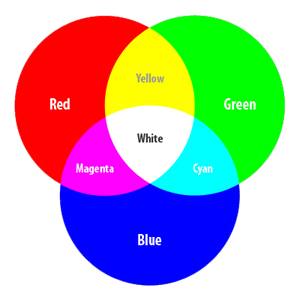
\includegraphics[width=0.48\textwidth]{1}
    \caption{Mezcla de colores aditiva}
    \label{fig:my_label}
\end{figure}

Básicamente los colores se dividen en primarios, secundarios y terciarios es posible a partir de combinaciones que se obtienen por la superposición de ondas con longitudes que se extienden a través de todo el espectro visible diferentes colores. Por ejemplo el amarillo, este es una mezcla de dos colores primarios rojo y verde. Se puede observar claramente como la mezcla de los colores primarios como lo son el rojo, azul y verde al superponerse abarcan todas las longitudes de onda posibles dando como resultado el color blanco o lo que se conoce como luz blanca. 
\\
Cuando se realizaba experimentalmente en el laboratorio la anulación de uno de los tres colores o sombras podíamos notar que esta suma de colores nos mostraba siempre un color secundario o derivado, al mezclar todos los colores obteníamos la luz blanca.
\\
La rapidez de la luz en el vacío es la misma para todas las longitudes de onda, pero la rapidez en una sustancia material es diferente para distintas longitudes de onda. En consecuencia, el índice de refracción de un material depende de la longitud de onda.







\section{(5.6.2) Ley de Snell}
\subsection{Análisis}
\subsubsection{}

\begin{table}[h!]
\begin{center}
\begin{tabular}{ |c|c|c| } 
 \hline
 Ángulo de Incidencia ($^{\circ})$ & Ángulo de Refracción ($^{\circ}$)& Índice de Refracción calculado\\ 
 \hline
 25 & 25 & 1.53  \\ 
 10 & 14 & 1.25  \\ 
 28 & 26 & 1.44  \\
 \hline
 & Promedio: & 1.41 \\
 \hline
\end{tabular}
\caption{ \emph{Angulos de incidencia y refracción para el trapezoide.}}
\label{table:1}
\end{center}
\end{table}



\subsubsection{}
Valor teorico para el indice de refraccción del acrilico
\begin{equation}
    n=1.25
\end{equation}

\begin{equation}
    \% Error = \frac{|Valor \ esperado-Valor \ experimental|}{Valor esperado}*100\%
\end{equation}

\begin{equation}
    \% Error =6\%
\end{equation}

Nota: Se observó un error relativamente bajo por lo que se concluyen que los datos tomados han sido de confianza para este experimento.

\begin{equation}
    incertidumbre=1.5 – 1.41 = 0.09
\end{equation}
\begin{equation}
    incertidumbre = 1.5+ 0.09 = 1.59 - incertidumbre= 1.5 – 0.09 = 1.41  
\end{equation}

\subsubsection{}
Cuando un rayo de luz llega a una superficie reflectora formando un angulo de incidencia $\theta_{i}$ con la normal a dicha superficie, se refleja en la superficie formando un angulo de reflexion $\theta_{r}$ con la misma normal.
\subsubsection{}

Dado que en las muestras tomadas en el laboratorio escribimos el angulo critico partiendo desde la normal  $\frac{\theta}{2}$, para este caso tomaremos ese mismo  $\frac{\theta}{2}$ conociendo que el valor del angulo critico  $\theta=90^{\circ}$ por ende  $\frac{\theta}{2}=45^{\circ}$.

\begin{table}[h!]
\begin{center}
\begin{tabular}{ |c|c|c|c| } 
 \hline
 N & Ángulo crítico$_{exp.}$ ($^{\circ}$) & Ángulo crítico$_{teo.}$ & \%Error\\ 
 \hline
 1 & 42.0  & 45 & 6.6\\ 
 2 & 45.0  & 45 & 0.0\\ 
 3 & 42.5  & 45 & 5.5\\
 \hline
\end{tabular}
\caption{ \emph{Calculo del ángulo crítico de un trapezoide.}}
\label{table:1}
\end{center}
\end{table}

\begin{table}[h!]
\begin{center}
\begin{tabular}{ |c|c|c|c| } 
 \hline
 Color & Ángulo crítico$_{exp.}$ ($^{\circ}$) & Ángulo crítico$_{teo.}$ & \%Error\\ 
 \hline
 Rojo & 38.5  & 45 & 14.4\\ 
 Azul & 36.0  & 45 & 20.0\\ 
 Verde& 34.0  & 45 & 24.9\\
 \hline
\end{tabular}
\caption{ \emph{Calculo del ángulo crítico de un trapezoide, colores.}}
\label{table:1}
\end{center}
\end{table}

\subsubsection{}
A medida que el angulo del rayo incidente se acerca al angulo critico , este empezara a tomar una mayor intensidad luminosa hasta que dado el punto en el que el rayo incidente llegue a su angulo critico el rayo que se refracta toma un nivel de luminosidad muy similar al rayo incidente.

\subsubsection{}
Aunque todos los colores tienen la misma velocidad de propagación en el aire y en el vacio, esto no ocurre en ciertos materiales.
\\
Debido a que (en un medio dispersivo) el índice de refracción varía con la frecuencia, luces de distintos colores sufrirán una mayor o menor refracción al atravesar estos medios. La luz roja, por ejemplo, sufre una menor desviación que la violeta produciéndose la separación de los distintos colores.
\\
Lo cual pudimos corroborar en el experimento ya que cada color presente un angulo critico distinto .



\section{(5.6.3) Óptica Geométrica}
\subsection{Análisis}

\begin{table}[h!]
\begin{center}
\begin{tabular}{ |c|c|c|c|c| } 
 \hline
 D. ima-obj (cm) & D. len-obj (cm)& D. len-ima (cm) & Tam. obj & Tam. ima (cm)\\ 
 \hline
 100 & 87.5	 & 12.5	& 4	&  0.5	\\ 
 90  & 88.5	 & 12.8	& 4	&  0.8	\\ 
 80  & 67.3	 & 13.1	& 4	&  1.0	\\
 70  & 66.5	 & 13.7	& 4	&  1.2	\\
 60  & 47.3	 & 14.5	& 4	&  1.4	\\
 50  & 33.5	 & 16.5	& 4	&  1.6	\\
 \hline
\end{tabular}
\caption{ \emph{Distancia más pequeña entre la lente y la imagen.}}
\label{table:1}
\end{center}
\end{table}


\begin{table}[h!]
\begin{center}
\begin{tabular}{ |c|c|c|c|c| } 
 \hline
 D. ima-obj (cm) & D. len-obj (cm)& D. len-ima (cm) & Tam. obj & Tam. ima (cm)\\ 
 \hline
 100 & 12.5  & 87.5	& 4	&  14.5	\\ 
 90  & 12.7	 & 77.5	& 4	&  13.0	\\ 
 80  & 13.0	 & 67.0	& 4	&  10.5	\\
 70  & 14.0	 & 56.6	& 4	&  8.5	\\
 60  & 14.5	 & 46.0	& 4	&  7.0	\\
 50  & 15.5	 & 34.5	& 4	&  4.5	\\
 \hline
\end{tabular}
\caption{ \emph{Distancia más grande entre la lente y la imagen.}}
\label{table:1}
\end{center}
\end{table}

$\\$
$\\$
$\\$
$\\$

\subsubsection{}
Calcule 1/dO y 1/di para todos los valores de la Tabla 5 y 6
\begin{table}[h!]
\begin{center}
\begin{tabular}{ |c|c|c| } 
 \hline
 1/dO (cm$^{-1}$) & 1/di (cm$^{-1}$) & f$_{exp.}$(cm)\\ 
 \hline
 0.011  & 0.080  & 10.9	\\ 
 0.011  & 0.078	 & 11.2	\\ 
 0.015  & 0.076	 & 11.0	\\
 0.015  & 0.073	 & 11.4	\\
 0.021  & 0.069	 & 11.1	\\
 0.030  & 0.061	 & 11.1	\\
 \hline
  & Promedio: & 11.1 \\
 \hline
\end{tabular}
\caption{ \emph{Distancia más grande entre la lente y la imagen.}}
\label{table:1}
\end{center}
\end{table}

\begin{table}[h!]
\begin{center}
\begin{tabular}{ |c|c|c| } 
 \hline
 1/dO (cm$^{-1}$) & 1/di (cm$^{-1}$) & f$_{exp.}$ (cm)\\ 
 \hline
 0.080  & 0.011  &	10.9\\ 
 0.079  & 0.013	 &	10.9\\ 
 0.077  & 0.015	 &	10.9\\
 0.071  & 0.018	 &	11.2\\
 0.069  & 0.022	 &	11.0\\
 0.065  & 0.029	 & 	10.7\\
 \hline
  & Promedio: & 10.9 \\ 
 \hline
\end{tabular}
\caption{ \emph{Distancia más grande entre la lente y la imagen.}}
\label{table:1}
\end{center}
\end{table}


\subsubsection{}
Grafique en Excel l/dO (eje Y) y 1/di (eje X). \emph{(Vease la Figura 2 y 3)}

\begin{center}
\begin{figure}[!ht]
    \centering
    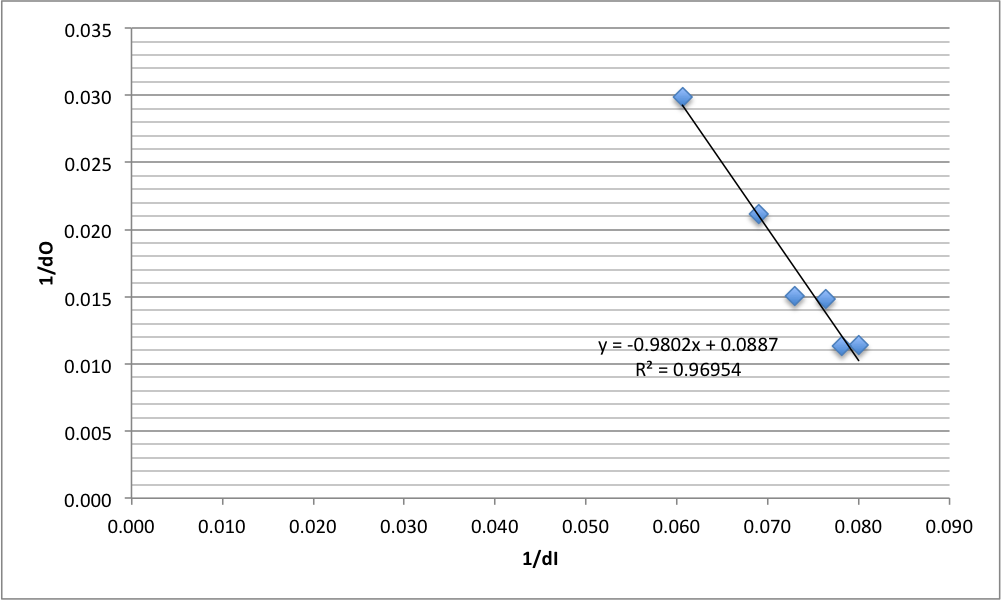
\includegraphics[width=1\textwidth]{2.png}
    \caption{Distancia más pequeña entre la lente y la imagen, Tabla 7.}
    \label{fig:my_label}
\end{figure}
\end{center}

\begin{center}
\begin{figure}[!ht]
    \centering
    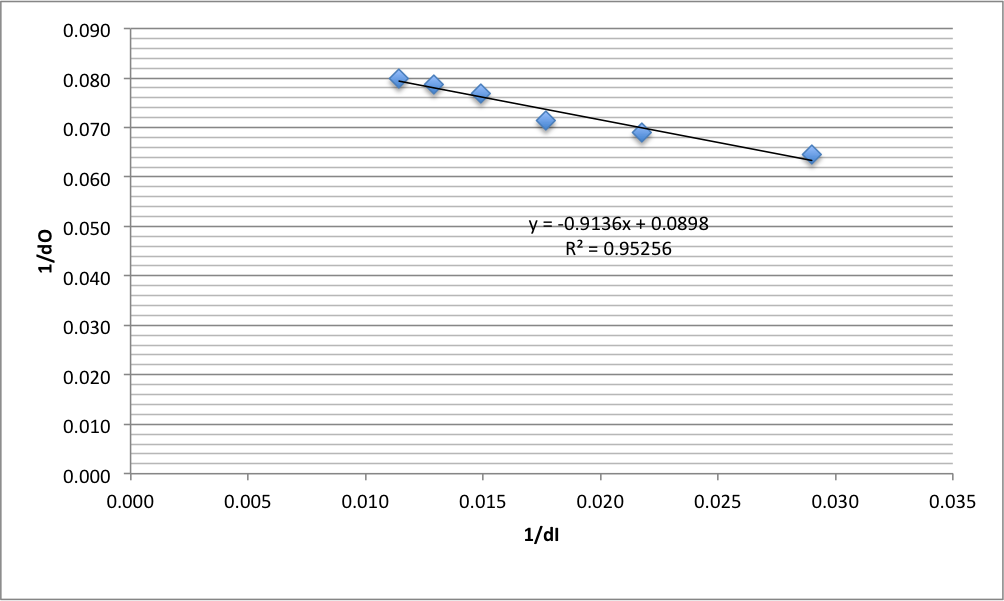
\includegraphics[width=1\textwidth]{3.png}
    \caption{Distancia más grande entre la lente y la imagen Tabla 8.}
    \label{fig:my_label}
\end{figure}
\end{center}

\subsubsection{}
\begin{equation}
    y_{1}=-0.9802x+0.0887
\end{equation}
\begin{equation}
    y_{2}=-0.9136x+0.0898
\end{equation}

La ecuación teorica de la distancia focal es:
\begin{equation}
    \frac{1}{f}=\frac{1}{dO}+\frac{1}{di}
\end{equation}

Forma general lineal
\begin{equation}
    y=mx\pm b
\end{equation}

Comparando, se obtien la siguiente relación:
\begin{equation}
    \frac{1}{dO}=y \ \ \ \ \ \frac{1}{di}=x \ \ \ \ \ \frac{1}{f}=b
\end{equation}
Por lo tanto, el promedio de la distancia focal experimental \emph{(Vease Tabla 7 y 8)} que se obtiene para la distancia más pequeña entre la lente y la imagen es igual a:

\begin{equation}
    f_{1}=11.1 \ cm \ \ = \ \ 111 \ mm
\end{equation}
La distancia según el fabricante es de:
\begin{equation}
    f=100 \ mm
\end{equation}

Por lo tanto el error porcentual es:
\begin{equation}
    \% Error=11\%
\end{equation}

el promedio de la distancia focal experimental \emph{(Vease Tabla 7 y 8)} que se obtiene para la distancia más grande entre la lente y la imagen es igual a:

\begin{equation}
    f_{2}=10.9 \ cm \ \ = \ \ 109 \ mm
\end{equation}

La distancia según el fabricante es de:
\begin{equation}
    f=100 \ mm
\end{equation}

Por lo tanto el error porcentual es:
\begin{equation}
    \% Error=9\%
\end{equation}


\subsubsection{}
(\emph{Vease Tabla  9 y 10})

\begin{table}[h!]
\begin{center}
\begin{tabular}{ |c|c| } 
 \hline
 Magnificación: (M=di/dO) & M$_{esp.}$\\ 
 \hline
 & 0.143    	\\ 
 & 0.145  	 	\\ 
 & 0.195 	 	\\
 & 0.206 	 	\\
 & 0.307  	 	\\
 & 0.493  	 	\\
 \hline
  Promedio: & 0.248 \\

 \hline
\end{tabular}
\caption{ \emph{Distancia más pequeña entre la lente y la imagen.}}
\label{table:1}
\end{center}
\end{table}

\begin{table}[h!]
\begin{center}
\begin{tabular}{ |c|c| } 
 \hline
 Magnificación: (M=di/dO) & M$_{esp.}$ \\ 
 \hline
 & 7.000 	    \\ 
 & 6.102  	 	\\ 
 & 5.154  	 	\\
 & 4.043  	 	\\
 & 3.172  	 	\\
 & 2.226  	 	\\
 \hline
  Promedio: & 4.616  \\
 \hline
\end{tabular}
\caption{ \emph{Distancia más grande entre la lente y la imagen.}}
\label{table:1}
\end{center}
\end{table}


\subsubsection{}
(\emph{Vease Tabla 11 y 12})
\begin{table}[h!]
\begin{center}
\begin{tabular}{ |c|c| } 
 \hline
 Magnificación: (T=Ti/TO) & M$_{exp.}$ \\ 
 \hline
 & 0.125 	    \\ 
 & 0.200  	 	\\ 
 & 0.250  	 	\\
 & 0.300  	 	\\
 & 0.350  	 	\\
 & 0.400  	 	\\
 \hline
  Promedio: & 0.271  \\

 \hline
\end{tabular}
\caption{ \emph{Distancia más pequeña entre la lente y la imagen.}}
\label{table:1}
\end{center}
\end{table}

\begin{table}[h!]
\begin{center}
\begin{tabular}{ |c|c| } 
 \hline
 Magnificación: (T=Ti/TO) & M$_{exp.}$ \\ 
 \hline
 & 3.625 	    \\ 
 & 3.250  	 	\\ 
 & 2.625  	 	\\
 & 2.125  	 	\\
 & 1.750  	 	\\
 & 1.125  	 	\\
 \hline
  Promedio: & 3.417  \\

 \hline
\end{tabular}
\caption{ \emph{Distancia más grande entre la lente y la imagen.}}
\label{table:1}
\end{center}
\end{table}

\subsubsection{}
Para representar el error porcentual entre el \emph{Valor experimental} y el \emph{Valor esperado} tomado en la medida se sigue la siguiente ecuación:

\begin{equation}
    \% Error = \frac{|Valor \ esperado-Valor \ experimental|}{Valor esperado}*100\%
\end{equation}

Para la distancia más pequeña entre la lente y la imagen tenemos:

\begin{equation}
    \% Error = \frac{|0.248-0.271|}{0.248}*100\%    
\end{equation}

\begin{equation}
    \% Error = 9.27\%
\end{equation}

Para la distancia más grande entre la lente y la imagen tenemos:

\begin{equation}
    \% Error = \frac{|4.616-3.417|}{4.16}*100\%    
\end{equation}

\begin{equation}
    \% Error = 25,97\%
\end{equation}

\subsubsection{}
La imagen real es aquella que se forma cuando, tras pasar por el sistema óptico, los rayos de luz son convergentes.
\\
Esta imagen no la podemos percibir directamente con nuestro sentido de la vista, pero puede registrarse colocando una pantalla en el lugar donde convergen los rayos.
\\
La formación de imagenes que se pudo observar en el laboratorio através de un lente convexo sugiere que aquella imagenes que se forman cuando los rayos de luz que describen una trayectoria chocan contra una pared y permite la visualización de una imagen real y con modificación en su tamaño, dependiendo de la posición del objeto (fuente de luz). 
\\
Al realizar un análisis de la trayectorias de los rayos en una lente convergente y la con base en los conceptos básicos adquiridos en el laboratorio identificamos que la imagen no fue virtual, tipo de lente, y tampoco estaba invertida, a nivel experimental se pudo comprobar que la lente era convergente y la formación de la imagen real.


\section{Bibliografia}
[1] https://es.wikipedia.org/wiki/Imagen$_(óptica)$
$\\$
$[2]$ https://www.morehouse.edu/facstaff/cmoore/Phy254
\\
LawsOfGeometricalOptics.html
$\\$
$[3]$ Raymond A. Serway Physics for Scientists and Engineers with Modern Physics. 
$\\$
$[4]$ Sears and Zemansky's University Physics.
$\\$
[5] Eugene Hecht, Optics
\end{document}

